En este cap�tulo de detallan las pruebas de rendimiento de la red, basado en los par�metros \mb mas relevantes de una linea serial.

\section{Resultados y an�lisis}

Se toma como m�trica de rendimiento  el porcentaje de respuesta Modbus, es decir, la relaci�n entre el n�mero de excepciones Modbus y el n�mero total de solicitudes hechas por el maestro. Las excepciones de no respuesta (\textit{Timeout}) son las que se consideran para el estudio de rendimiento, pues otros tipos de excepciones pueden estar asociadas al mal funcionamiento de los esclavos, y no la red inal�mbrica.



 Se asume que los esclavos posee un porcentaje de error sobre linea  serial menor al 1\%  para entrega y menor a 2\% parra respuesta, seg�n las especificaciones de equipos Modbus para linea serial. Se asume que las antenas son omnidireccionales dispuestas verticalmente.
 
 \subsection{Rendimiento y tiempo de muestreo}

La tabla \ref{Res: Scan} presenta los resultados de las mediciones para distintos tiempos de muestreo del maestro. 
\begin{table}[H]
\centering
\begin{tabular}{|c|c|c|c|c|c|c|}
\hline 
 & \multicolumn{5}{c|}{\% de error por esclavos } &   \\ 
\hline 
Tiempo de Muestro [s] &  ID 1 &   ID 2 &  ID 150 & ID 151 & ID 153 & \textbf{Promedio} \% \\ 
\hline 
10 & 0,21 & 0,74 & 0,00 & 0,11 & 0,89 & \textbf{0,39} \\ 
\hline 
5 & 0,10 & 0,00 & 0,00 & 0,10 & 0,10 & \textbf{0,06} \\ 
\hline 
2 & 0,00 & 0,10 & 0,00 & 0,10 & 0,30 & \textbf{0,10} \\ 
\hline 
1 & 0,20 & 0,00 & 0,00 & 0,30 & 0,30 & \textbf{0,16 }\\ 
\hline 
\textbf{Promedio por ID}& \textbf{0,12} & \textbf{0,21 }& \textbf{0,00 }& \textbf{0,17} &\textbf{ 0,39 }&\textbf{ 0,18} \\ 
\hline 
\end{tabular} 
\caption{Porcentajes de error para variaciones en el tiempo de muestro}\label{Res: Scan}
\end{table}

%\begin{table}
\subsection{Rendimiento y n�mero de variables}

La tabla \ref{Res: var} presenta los resultados de las mediciones para distintos n�meros de variables. 
\begin{table}[H]
\centering
\begin{tabular}{|c|c|c|c|c|c|c|}
\hline 
 & \multicolumn{5}{c|}{\% de error por esclavos } &   \\ 
\hline 
N�mero de variables [s] &  ID 1 &   ID 2 &  ID 150 & ID 151 & ID 153 & \textbf{Promedio} \% \\ 
\hline 
50 & 0,10 & 0,00 & 0,00 & 0,10 & 0,10 & \textbf{0,06} \\ 
\hline 
100 & 0,34 & 0,25 & 0,00 & 0,08 & 0,34 & \textbf{0,20} \\ 
\hline 
150 & 0,19 & 0,00 & 0,09 & 0,00 & 0,00 & \textbf{0,06} \\ 
\hline 
200 & 0,30 & 0,30 & 0,00 & 0,15 & 0,23 & \textbf{0,20 }\\ 
\hline 
250 & 0,20 & 0,29 & 0,00 & 0,10 & 0,59 & \textbf{0,23 }\\ 
\hline 
\textbf{Promedio por ID}& \textbf{0,23} & \textbf{0,17 }& \textbf{0,02 }& \textbf{0,09} &\textbf{ 0,25}&\textbf{ 0,15} \\ 
\hline 
\end{tabular} 
\caption{Porcentajes de error para variaciones en el tiempo de muestro}\label{Res: var}
\end{table}

\subsection{Rendimiento y tasa de baudios}

La tabla \ref{Res: bad} presenta los resultados de las mediciones para distintas tasa de baudios. 
\begin{table}[H]
\centering
\begin{tabular}{|c|c|c|c|c|c|c|}
\hline 
 & \multicolumn{5}{c|}{\% de error por esclavos } &   \\ 
\hline 
Tasa de baudios [s] &  ID 1 &   ID 2 &  ID 150 & ID 151 & ID 153 & \textbf{Promedio} \% \\ 
\hline 
2400 & 0,86	 & 2,67 & 1,62 & 0,48& 4,29 & \textbf{1,98} \\ 
\hline 
4800 & 0,32& 0,24 & 0,49 & 0,41 & 1,78 & \textbf{0,65} \\ 
\hline 
9600 & 0,17 & 0,67 & 0,42 & 0,17 & 3,74 & \textbf{1,03} \\ 
\hline 
19200 & 0,19 & 4,38 & 0,37 & 0,19 & 4,29 & \textbf{1,88 }\\ 
\hline 
38400 & 0,29 & 0,46 & 0,09 & 0,19 & 0,56 & \textbf{0,30 }\\ 
\hline 
\textbf{Promedio por ID}& \textbf{0,34} & \textbf{1,68 }& \textbf{0,60 }& \textbf{0,28} &\textbf{ 2,93}&\textbf{ 1,17} \\ 
\hline 
\end{tabular} 
\caption{Porcentajes de error para variaciones en la tasa de baudios}\label{Res: top}
\end{table}
%%
%%
\subsection{Rendimiento y topolog�a}

La tabla \ref{Res: bad} presenta los resultados de las mediciones para distintas topolog�as. 
\begin{table}[H]
\centering
\begin{tabular}{|c|c|c|c|c|c|c|}
\hline 
 & \multicolumn{5}{c|}{\% de error por esclavos } &   \\ 
\hline 
Topolog�a [s] &  ID 1 &   ID 2 &  ID 150 & ID 151 & ID 153 & \textbf{Promedio} \% \\ 
\hline 
1 & 12,20 & 2,60 & 0,25 & 0,25 & 2,60 & \textbf{3,58} \\ 
\hline 
2 & 3,24& 0,16& 0,08 & 0,32& 11,35 & \textbf{3,03} \\ 
\hline 
3 & 0,07 & 0,14 & 0,00 & 0,14 & 0,00 & \textbf{0,07} \\ 
\hline 
\textbf{Promedio por ID}& \textbf{5,17} & \textbf{0,97 }& \textbf{0,11 }& \textbf{0,24} &\textbf{4,65}&\textbf{ 2,23} \\ 
\hline 
\end{tabular} 
\caption{Porcentajes de error para variaciones en la topolg�a}\label{Res: top}
\end{table}
%
Para las topolog�as presentadas en las figuras \ref{topo1}, \ref{topo2} y\ref{topo3}.
%
\begin{figure}[H]
\centering
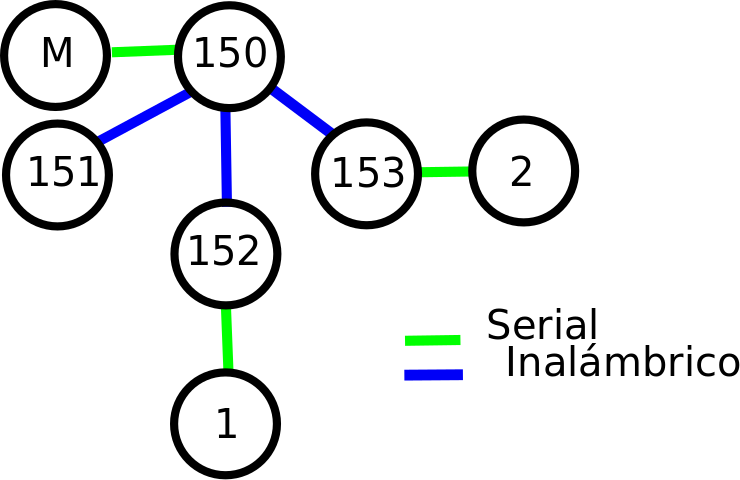
\includegraphics[scale=0.3]{images/topo1.png}
\caption{Topolog�a 1 de prueba}\label{topo1}
\end{figure}

\begin{figure}[H]
\centering
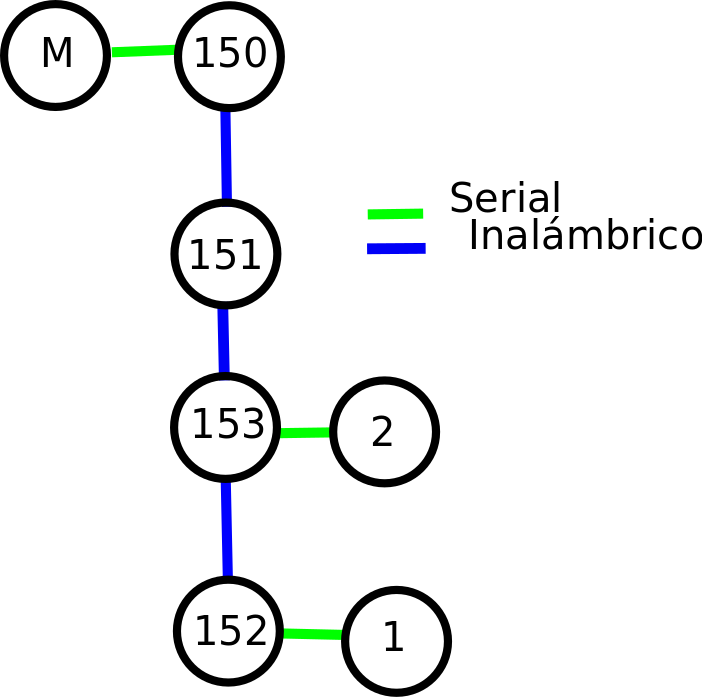
\includegraphics[scale=0.3]{images/topo2.png}
\caption{Topolog�a 2 de prueba}\label{topo1}
\end{figure}

\begin{figure}[H]
\centering
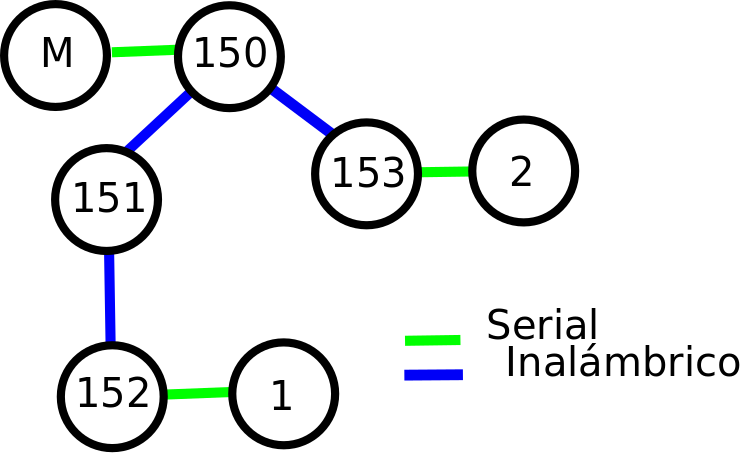
\includegraphics[scale=0.3]{images/topo3.png}
\caption{Topolog�a 3 de prueba}\label{topo1}
\end{figure}